% File: lecture_3.tex
\section{Advanced Entropy Coding \& Extensions}

\begin{center}
\textbf{Lecture 3: Beyond Huffman -- Advanced Entropy Coding Methods}
\end{center}

\subsection{Introduction \& Motivation}

\begin{importantbox}
\textbf{Recall Huffman Coding Limitations:}
\begin{itemize}
    \item \textbf{Integer code lengths}: Cannot reach entropy bound for highly skewed distributions
    \item \textbf{Static vs. Adaptive}: Standard Huffman requires prior knowledge of probabilities
    \item \textbf{Codebook overhead}: Need to transmit/store the coding tree
    \item \textbf{Symbol-by-symbol constraint}: Processes one symbol at a time
\end{itemize}
\end{importantbox}

\textbf{Lecture Roadmap:}
\begin{enumerate}
    \item \textbf{Framework}: Coding taxonomy and conceptual organization
    \item \textbf{Historical methods}: Shannon \& Shannon-Fano coding
    \item \textbf{Practical improvements}: Canonical and Adaptive Huffman
    \item \textbf{Next generation}: Arithmetic coding paradigm
    \item \textbf{Synthesis}: Comparison and forward look
\end{enumerate}

\subsection{Coding Taxonomy \& Framework}

\begin{definitionbox}
\textbf{Coding Taxonomy:} Classification of compression methods based on key characteristics
\end{definitionbox}

\begin{center}
\begin{tikzpicture}[node distance=1.5cm]
\node (compression) [rectangle, draw=black, thick, fill=blue!10, minimum width=3cm, minimum height=1cm] {\textbf{Compression Methods}};
\node (entropy) [below left=of compression, rectangle, draw=black, thick, fill=green!10, minimum width=2.5cm] {Entropy Coding};
\node (dictionary) [below right=of compression, rectangle, draw=black, thick, fill=orange!10, minimum width=2.5cm] {Dictionary Coding};
\node (shannon) [below=of entropy, rectangle, draw=black, fill=green!5, text width=2cm, align=center] {Shannon Coding};
\node (shannonfano) [below=of shannon, rectangle, draw=black, fill=green!5, text width=2cm, align=center] {Shannon-Fano};
\node (huffman) [below=of shannonfano, rectangle, draw=black, fill=green!5, text width=2cm, align=center] {Huffman};
\node (arithmetic) [below=of huffman, rectangle, draw=black, fill=green!5, text width=2cm, align=center] {Arithmetic};

\draw[->, thick] (compression) -- (entropy);
\draw[->, thick] (compression) -- (dictionary);
\draw[->] (entropy) -- (shannon);
\draw[->] (shannon) -- (shannonfano);
\draw[->] (shannonfano) -- (huffman);
\draw[->] (huffman) -- (arithmetic);
\end{tikzpicture}
\end{center}

\textbf{Key Dimensions in Coding Taxonomy:}

\begin{enumerate}
    \item \textbf{Modeling vs. Coding Separation:}
    \begin{itemize}
        \item \textbf{Modeling}: Probability estimation of symbols
        \item \textbf{Coding}: Assigning bit sequences based on probabilities
    \end{itemize}
    
    \item \textbf{Static vs. Adaptive vs. Universal:}
    \begin{itemize}
        \item \textbf{Static}: Fixed probabilities known in advance
        \item \textbf{Adaptive}: Probabilities updated during encoding
        \item \textbf{Universal}: Adapts to unknown distributions
    \end{itemize}
    
    \item \textbf{Block Codes vs. Stream Codes:}
    \begin{itemize}
        \item \textbf{Block}: Fixed-length input blocks
        \item \textbf{Stream}: Continuous data processing
    \end{itemize}
    
    \item \textbf{Symbol-by-Symbol vs. Message-Wide:}
    \begin{itemize}
        \item \textbf{Symbol-by-symbol}: Each symbol coded independently (Huffman)
        \item \textbf{Message-wide}: Entire message coded as one unit (Arithmetic)
    \end{itemize}
\end{enumerate}

\subsection{Shannon Coding (1948)}

\begin{definitionbox}
\textbf{Shannon Coding:} A constructive method derived from Shannon's source coding theorem:
\[
l_i = \lceil -\log_2 p_i \rceil
\]
where $p_i$ is the probability of symbol $i$.
\end{definitionbox}

\begin{examplebox}
\textbf{Example:} Given symbols with probabilities:
\begin{center}
\begin{tabular}{c|c|c}
Symbol & Probability & $-\log_2 p_i$ \\
\hline
A & 0.5 & 1.0 \\
B & 0.25 & 2.0 \\
C & 0.125 & 3.0 \\
D & 0.125 & 3.0 \\
\end{tabular}
\end{center}

\textbf{Shannon code construction:}
\begin{enumerate}
    \item Calculate lengths: $l_A = \lceil 1.0 \rceil = 1$, $l_B = 2$, $l_C = 3$, $l_D = 3$
    \item Sort by probability (decreasing)
    \item Assign cumulative probabilities: $F_A=0$, $F_B=0.5$, $F_C=0.75$, $F_D=0.875$
    \item Convert $F_i$ to binary with $l_i$ bits:
    \begin{itemize}
        \item A: $0.0_2 \rightarrow 0$
        \item B: $0.5_{10} = 0.1_2 \rightarrow 10$
        \item C: $0.75_{10} = 0.11_2 \rightarrow 110$
        \item D: $0.875_{10} = 0.111_2 \rightarrow 111$
    \end{itemize}
\end{enumerate}
\textbf{Expected length:} $L = 0.5\times1 + 0.25\times2 + 0.125\times3 + 0.125\times3 = 1.75$ bits/symbol
\end{examplebox}

\begin{importantbox}
\textbf{Properties of Shannon Coding:}
\begin{itemize}
    \item \textbf{Constructive proof}: Demonstrates Kraft-McMillan inequality
    \item \textbf{Simple to compute}: Direct from probabilities
    \item \textbf{Not optimal}: Unlike Huffman, doesn't minimize expected length
    \item \textbf{Theoretical importance}: Foundation for Shannon's theorem
\end{itemize}
\end{importantbox}

\subsection{Shannon-Fano Coding (1949)}

\begin{definitionbox}
\textbf{Shannon-Fano Coding:} A top-down recursive splitting method developed independently by Shannon and Fano.
\end{definitionbox}

\begin{algorithm}
\caption{Shannon-Fano Coding Algorithm}
\begin{algorithmic}[1]
\REQUIRE Symbols with probabilities $p_1 \geq p_2 \geq \cdots \geq p_n$
\ENSURE Prefix code for each symbol
\STATE Sort symbols by decreasing probability
\STATE \textbf{function} SF($symbols$)
    \IF{$|symbols| = 1$}
        \RETURN (assign empty code)
    \ENDIF
    \STATE Split $symbols$ into two subsets $S_1$ and $S_2$ with nearly equal total probabilities
    \STATE Append '0' to codes of symbols in $S_1$
    \STATE Append '1' to codes of symbols in $S_2$
    \STATE SF($S_1$)
    \STATE SF($S_2$)
\STATE \textbf{end function} % FIXED: Changed \ENDFUNCTION to proper syntax
\end{algorithmic}
\end{algorithm}

\begin{examplebox}
\textbf{Example:} Same symbols as before:
\begin{center}
\begin{tabular}{c|c}
Symbol & Probability \\
\hline
A & 0.5 \\
B & 0.25 \\
C & 0.125 \\
D & 0.125 \\
\end{tabular}
\end{center}

\textbf{Construction:}
\begin{enumerate}
    \item Split 1: $\{A\}(0.5)$ vs $\{B,C,D\}(0.5)$ → A:0, others:1
    \item Split 2: $\{B\}(0.25)$ vs $\{C,D\}(0.25)$ → B:10, others:11
    \item Split 3: $\{C\}(0.125)$ vs $\{D\}(0.125)$ → C:110, D:111
\end{enumerate}

\textbf{Codes:} A=0, B=10, C=110, D=111 \\
\textbf{Expected length:} Same as Huffman in this case: 1.75 bits/symbol
\end{examplebox}

\begin{importantbox}
\textbf{Historical Note:} Shannon-Fano coding was developed before Huffman coding (1952). While simpler conceptually, it is \textbf{not always optimal}. Huffman's bottom-up approach guarantees optimality for given probabilities.
\end{importantbox}

\subsection{Canonical Huffman Codes}

\begin{definitionbox}
\textbf{Canonical Huffman Code:} A Huffman code where codes are assigned in a specific canonical (standard) form, enabling more efficient representation and faster decoding.
\end{definitionbox}

\begin{algorithm}
\caption{Canonical Huffman Construction}
\begin{algorithmic}[1]
\REQUIRE Symbol code lengths $l_i$ from standard Huffman
\ENSURE Canonical Huffman codes
\STATE Sort symbols by: (1) code length $l_i$, (2) symbol value
\STATE Assign first code: $code = 0$ (in binary with $l_{min}$ bits)
\FOR{each symbol in sorted order}
    \STATE Assign current $code$ to symbol
    \STATE Increment $code$ by 1
    \IF{next symbol has longer code length}
        \STATE Left-shift $code$ by difference in lengths
    \ENDIF
\ENDFOR
\end{algorithmic}
\end{algorithm}

\begin{examplebox}
\textbf{Example:} Suppose Huffman gives these lengths:
\begin{center}
\begin{tabular}{c|c|c}
Symbol & Length & Original Huffman \\
\hline
A & 2 & 00 \\
B & 3 & 010 \\
C & 3 & 011 \\
D & 3 & 100 \\
E & 4 & 1010 \\
F & 4 & 1011 \\
\end{tabular}
\end{center}

\textbf{Canonical construction:}
\begin{enumerate}
    \item Sort: A(2), B(3), C(3), D(3), E(4), F(4)
    \item Start: A gets code 00 (binary 0 in 2 bits)
    \item Increment: B gets 010 (binary 2 in 3 bits: 010)
    \item Increment: C gets 011 (binary 3: 011)
    \item Increment: D gets 100 (binary 4: 100)
    \item For E: length increases to 4, so left-shift: 100 → 1000
    \item Increment: F gets 1001
\end{enumerate}

\textbf{Canonical codes:} A=00, B=010, C=011, D=100, E=1000, F=1001
\end{examplebox}

\begin{importantbox}
\textbf{Advantages of Canonical Huffman:}
\begin{itemize}
    \item \textbf{Compact representation}: Only need to store code lengths, not the full tree
    \item \textbf{Fast decoding}: Use table-based lookup instead of tree traversal
    \item \textbf{Standardized}: Used in DEFLATE (ZIP, gzip), JPEG, PNG, MPEG
\end{itemize}

\textbf{Transmission:} Send only: $\langle$symbol count, lengths$\rangle$ instead of full tree
\end{importantbox}

\subsection{Adaptive Huffman Coding}

\begin{definitionbox}
\textbf{Adaptive Huffman Coding:} Dynamically updates the Huffman tree as symbols are processed, requiring only one pass over the data.
\end{definitionbox}

\textbf{Key Algorithms:}
\begin{itemize}
    \item \textbf{FGK Algorithm} (Faller, Gallager, Knuth, 1978)
    \item \textbf{Vitter's Algorithm} (1987) - more efficient
\end{itemize}

\begin{importantbox}
\textbf{How it works:}
\begin{enumerate}
    \item Start with empty tree or initial estimates
    \item For each symbol:
    \begin{itemize}
        \item Encode using current tree
        \item Update symbol frequency
        \item Reconstruct/update tree incrementally
    \end{itemize}
    \item Sibling property maintained for optimality
\end{enumerate}
\end{importantbox}

\textbf{Applications:} Early UNIX compress utility, network protocols where distribution changes.

\subsection{Arithmetic Coding: The Paradigm Shift}

\begin{definitionbox}
\textbf{Arithmetic Coding:} Encodes an entire message into a single fractional number in the interval $[0,1)$, approaching the entropy bound very closely.
\end{definitionbox}

\textbf{Core Idea:} Represent messages as subintervals of $[0,1)$:

\begin{center}
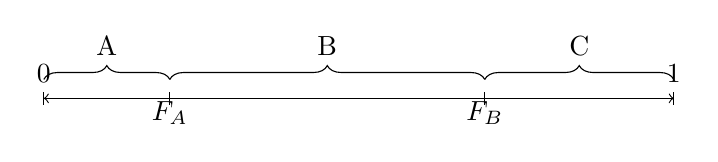
\begin{tikzpicture}[scale=0.8]
\draw[<->] (0,0) -- (10,0);
\draw (0,-0.1) -- (0,0.1) node[above] {0};
\draw (10,-0.1) -- (10,0.1) node[above] {1};
\draw (2,-0.1) -- (2,0.1) node[below] {$F_{A}$};
\draw (7,-0.1) -- (7,0.1) node[below] {$F_{B}$};
\draw[decorate,decoration={brace,amplitude=5pt}] (0,0.3) -- (2,0.3) node[midway,above=5pt] {A};
\draw[decorate,decoration={brace,amplitude=5pt}] (2,0.3) -- (7,0.3) node[midway,above=5pt] {B};
\draw[decorate,decoration={brace,amplitude=5pt}] (7,0.3) -- (10,0.3) node[midway,above=5pt] {C};
\end{tikzpicture}
\end{center}

\begin{algorithm}
\caption{Arithmetic Encoding Algorithm}
\begin{algorithmic}[1]
\REQUIRE Message $m = s_1 s_2 \dots s_k$, symbol probabilities $p_i$
\ENSURE Final interval $[low, high)$
\STATE $low \gets 0.0$, $high \gets 1.0$
\FOR{each symbol $s$ in $m$}
    \STATE $range \gets high - low$
    \STATE $high \gets low + range \times F_s$ \COMMENT{$F_s$: cumulative prob up to $s$}
    \STATE $low \gets low + range \times F_{s-1}$ \COMMENT{$F_{s-1}$: cumulative prob before $s$}
\ENDFOR
\RETURN any number in $[low, high)$
\end{algorithmic}
\end{algorithm}

\begin{examplebox}
\textbf{Example:} Encode message "CAB" with probabilities: A(0.5), B(0.25), C(0.25)

\begin{center}
\begin{tabular}{c|c|c}
Symbol & Probability & Cumulative \\
\hline
A & 0.5 & 0.5 \\
B & 0.25 & 0.75 \\
C & 0.25 & 1.0 \\
\end{tabular}
\end{center}

\textbf{Encoding:}
\begin{enumerate}
    \item Start: $[0, 1)$
    \item Process 'C': $[0.75, 1.0)$ \quad (C occupies $[0.75, 1.0)$)
    \item Process 'A': $range = 0.25$
        \begin{itemize}
            \item $low = 0.75 + 0.25 \times 0.0 = 0.75$
            \item $high = 0.75 + 0.25 \times 0.5 = 0.875$
            \item New interval: $[0.75, 0.875)$
        \end{itemize}
    \item Process 'B': $range = 0.125$
        \begin{itemize}
            \item $low = 0.75 + 0.125 \times 0.5 = 0.8125$
            \item $high = 0.75 + 0.125 \times 0.75 = 0.84375$
            \item Final interval: $[0.8125, 0.84375)$
        \end{itemize}
\end{enumerate}
\textbf{Output:} Any number in $[0.8125, 0.84375)$, e.g., 0.8125 in binary
\end{examplebox}

\begin{importantbox}
\textbf{Practical Implementation Issues:}
\begin{itemize}
    \item \textbf{Finite precision}: Use integer arithmetic with scaling
    \item \textbf{Renormalization}: Output bits when interval confined to one half
    \item \textbf{Carry-over}: Handle when interval spans midpoint
    \item \textbf{Termination}: Need special end-of-message symbol
\end{itemize}
\end{importantbox}

\textbf{Adaptive Arithmetic Coding:} Easier than adaptive Huffman - just update probabilities as you go!

\subsection{Comparison \& Synthesis}

% Fixed table to fit within margins
\begin{center}
\small % Use smaller font for table
\begin{tabular}{|p{2.5cm}|c|c|c|c|p{2.5cm}|}
\hline
\textbf{Method} & \textbf{Optimal?} & \textbf{Adaptive?} & \textbf{Complexity} & \textbf{Near Entropy?} & \textbf{Key Applications} \\
\hline
Shannon Coding & No & No & Low & No & Theoretical proofs \\
\hline
Shannon-Fano & No & No & Low & Sometimes & Historical \\
\hline
Huffman & Yes* & No & Low & Moderate & General purpose \\
\hline
Canonical Huffman & Yes* & No & Low & Moderate & DEFLATE, JPEG, PNG \\
\hline
Adaptive Huffman & Yes* & Yes & Medium & Moderate & Early compressors \\
\hline
Arithmetic Coding & \textbf{Near-opt} & \textbf{Yes} & \textbf{High} & \textbf{Yes (close)} & \textbf{JPEG2000, H.264, HEVC} \\
\hline
\end{tabular}
\end{center}
\smallskip
*Optimal for symbol-by-symbol coding given probabilities

\begin{importantbox}
\textbf{Key Insights:}
\begin{itemize}
    \item \textbf{Huffman vs. Arithmetic}: Huffman is simpler but has an "integer penalty"; Arithmetic approaches entropy bound
    \item \textbf{Modern standards}: Arithmetic coding (CABAC) used in video compression for 10-20\% better compression
    \item \textbf{Practical choice}: For general compression, Canonical Huffman (DEFLATE); for media, Arithmetic coding
    \item \textbf{The missing piece}: All these methods assume we have good probability estimates. Where do those come from?
\end{itemize}
\end{importantbox}

\subsection{Forward Look}

\textbf{The Complete Picture: What Comes Next?}

\begin{center}
\begin{tikzpicture}[node distance=1.8cm]
\node (lecture1) [rectangle, draw=black, thick, fill=blue!10, minimum width=3cm, minimum height=1cm] {\parbox{2.8cm}{\centering \textbf{Lecture 1}\\Huffman Coding}};
\node (lecture2) [below=of lecture1, rectangle, draw=black, thick, fill=green!10, minimum width=3cm, minimum height=1cm] {\parbox{2.8cm}{\centering \textbf{Lecture 2}\\Theory\\Entropy, Kraft-McMillan}};
\node (lecture3) [below=of lecture2, rectangle, draw=black, thick, fill=orange!10, minimum width=3cm, minimum height=1cm] {\parbox{2.8cm}{\centering \textbf{Lecture 3}\\Advanced Coding\\Arithmetic, Canonical}};
\node (lecture4) [below=of lecture3, rectangle, draw=black, thick, fill=red!10, minimum width=3cm, minimum height=1cm] {\parbox{2.8cm}{\centering \textbf{Lecture 4}\\Source Modeling\\Markov, Context}};
\node (lecture5) [below=of lecture4, rectangle, draw=black, thick, fill=purple!10, minimum width=3cm, minimum height=1cm] {\parbox{2.8cm}{\centering \textbf{Lecture 5}\\Dictionary Methods\\LZ Family}};

\draw[->, thick] (lecture1) -- (lecture2);
\draw[->, thick] (lecture2) -- (lecture3);
\draw[->, thick] (lecture3) -- (lecture4);
\draw[->, thick] (lecture4) -- (lecture5);
\end{tikzpicture}
\end{center}

\textbf{Next Lecture: Source Modeling and Statistical Dependence}
\begin{itemize}
    \item \textbf{The missing half}: We now know how to code efficiently, but where do the probabilities come from?
    \item \textbf{Real data has memory}: 'Q' is usually followed by 'U' in English text
    \item \textbf{Markov models}: Capturing dependencies between symbols
    \item \textbf{Context modeling}: Using past symbols to predict future ones
    \item \textbf{The modeling-coding separation}: Modern compressors separate these two tasks
\end{itemize}

\textbf{The Big Question for Next Time:}
\begin{center}
\fbox{\parbox{0.8\textwidth}{\centering
\textbf{If Arithmetic coding can get within 0.01 bits of entropy,\\ 
what's the real limit to compression?\\ 
The answer: It's not the coding, it's the \textit{modeling}!}}
}
\end{center}

\textbf{The Two Pillars of Compression (Revised View):}
\begin{center}
\begin{tikzpicture}[node distance=2cm]
\node (comp) [rectangle, draw=black, thick, minimum width=8cm, minimum height=2cm] {\textbf{Data Compression}};
\node (modeling) [below left=1cm of comp.south, rectangle, draw=red, thick, fill=red!5, minimum width=3.5cm, minimum height=1.2cm] {\parbox{3.2cm}{\centering \textbf{Modeling}\\Probability Estimation\\90\% of compression gain}};
\node (coding) [below=of comp, rectangle, draw=blue, thick, fill=blue!5, minimum width=3.5cm, minimum height=1.2cm] {\parbox{3.2cm}{\centering \textbf{Coding}\\Bit Assignment\\10\% of compression gain}};
\node (dictionary) [below right=1cm of comp.south, rectangle, draw=green, thick, fill=green!5, minimum width=3.5cm, minimum height=1.2cm] {\parbox{3.2cm}{\centering \textbf{Dictionary}\\Repetition-based\\Different approach}};

\draw[->, thick, red] (comp.south) -- (modeling);
\draw[->, thick, blue] (comp.south) -- (coding);
\draw[->, thick, green] (comp.south) -- (dictionary);

\node (modeltech) [below=0.5cm of modeling] {\parbox{3.2cm}{\centering Markov Models\\Context Modeling\\PPM}};
\node (codetech) [below=0.5cm of coding] {\parbox{3.2cm}{\centering Huffman\\Arithmetic\\Canonical}};
\node (dicttech) [below=0.5cm of dictionary] {\parbox{3.2cm}{\centering LZ77, LZ78\\LZW\\DEFLATE}};

\draw[red!50] (modeling) -- (modeltech);
\draw[blue!50] (coding) -- (codetech);
\draw[green!50] (dictionary) -- (dicttech);
\end{tikzpicture}
\end{center}

\begin{exercisebox}
\textbf{Exercise 3.1:} Given symbols with probabilities: A(0.4), B(0.3), C(0.2), D(0.1)
\begin{enumerate}[label=(\alph*)]
    \item Construct a Shannon code and compute its expected length
    \item Construct a Shannon-Fano code
    \item Compare with Huffman code from Lecture 2
\end{enumerate}
\end{exercisebox}

\begin{exercisebox}
\textbf{Exercise 3.2:} Convert the following Huffman code to canonical form:
\begin{center}
\begin{tabular}{c|c}
Symbol & Huffman Code \\
\hline
A & 0 \\
B & 100 \\
C & 101 \\
D & 110 \\
E & 1110 \\
F & 1111 \\
\end{tabular}
\end{center}
\end{exercisebox}

\begin{exercisebox}
\textbf{Exercise 3.3:} Encode the message "ABAC" using arithmetic coding with probabilities: A(0.6), B(0.3), C(0.1). Show each step.
\end{exercisebox}

\begin{exercisebox}
\textbf{Exercise 3.4: Thinking Ahead:} Consider the English phrase "THE QUICK BROWN FOX"
\begin{enumerate}[label=(\alph*)]
    \item If we use Huffman coding with letter frequencies, what's wrong with this approach?
    \item How might knowing that 'Q' is usually followed by 'U' help compression?
    \item Why would arithmetic coding be better than Huffman for this kind of data?
\end{enumerate}
\end{exercisebox}

\vspace{1cm}
\begin{center}
\rule{0.8\textwidth}{0.5pt}\\
\textbf{End of Lecture 3 -- Advanced Entropy Coding Methods}\\
\textbf{Next: Lecture 4 -- Source Modeling and Statistical Dependence}\\
\textit{We now have efficient coding methods. Next: Where do the probabilities come from?}
\end{center}
